%!=XeLatex
% !TEX encoding = UTF-8 Unicode
\documentclass[a4paper, 11pt, nofonts, nocap, fancyhdr, hyperref, UTF8]{ctexart}

\usepackage[margin=90pt]{geometry}
\usepackage{amsfonts}
% \usepackage{amsthm}
\usepackage{indentfirst}             % 首行缩进
\usepackage[perpage,symbol]{footmisc}% 脚注控制
\usepackage[sf]{titlesec}            % 控制标题
\usepackage{titletoc}                % 控制目录
\usepackage{fancyhdr}                % 页眉页脚
\usepackage{type1cm}                 % 控制字体大小
\usepackage{indentfirst}             % 首行缩进
\usepackage{makeidx}                 % 建立索引
\usepackage{textcomp}                % 千分号等特殊符号
\usepackage{layouts}                 % 打印当前页面格式
\usepackage{bbding}                  % 一些特殊符号
\usepackage{cite}                    % 支持引用
\usepackage{color,xcolor}            % 支持彩色文本、底色、文本框等
\usepackage{listings}                % 粘贴源代码
\usepackage{algorithm,algpseudocode, algorithmicx}
%\usepackage{algorithmic}
\usepackage{graphics}
\usepackage{graphicx}
\usepackage{epsfig}
%\usepackage[dvips]{graphicx}       % 将eps格式的图片放在figures目录下
%\usepackage[pdftex]{graphicx}      % \graphicspath{{figures/}}
\usepackage{multirow}
\usepackage{amsmath}
\usepackage{amstext}
%\usepackage[colorlinks,linkcolor=red]{hyperref}
\usepackage{subfigure}
\usepackage{float} %算法浮动体
\usepackage{xeCJK} % 使用xeCJK宏包

\lstloadlanguages{}                  % 所要粘贴代码的编程语言

% \setCJKmainfont[Mapping = fullwidth-stop, BoldFont={黑体-简}, ItalicFont={楷体-简}]{宋体-简}
% \setCJKsansfont[Mapping = fullwidth-stop, BoldFont={黑体-简}, ItalicFont={楷体-简}]{宋体-简}
% \setCJKmonofont[Mapping = fullwidth-stop, BoldFont={黑体-简}, ItalicFont={楷体-简}]{宋体-简}
%\setCJKmainfont{宋体}
%\setCJKsansfont{宋体}
%\setCJKmonofont{宋体}

\titleformat*{\section}{\Large \bf}
\titleformat*{\subsection}{\large \bf}

\CTEXoptions[today=small]

\pagestyle{plain}

% \newtheorem{example}{例}[section]             % 整体编号
% \newtheorem{theorem}{定理}[section]  % 按 section 编号
% %\newtheorem{proof}{证明}[section]
% \newtheorem{definition}{定义}[section]
% \newtheorem{axiom}{公理}
% \newtheorem{property}{性质}
% \newtheorem{proposition}{命题}
% \newtheorem{lemma}{引理}
% \newtheorem{corollary}{推论}
% \newtheorem{remark}{注解}
% \newtheorem{condition}{条件}
% \newtheorem{conclusion}{结论}
% \newtheorem{assumption}{假设}
% \floatname{algorithm}{算法}

% \renewcommand{\contentsname}{目录}     % 将Contents改为目录
% \renewcommand{\abstractname}{摘\ \ 要} % 将Abstract改为摘要
% \renewcommand{\refname}{参考文献}      % 将References改为参考文献
% \renewcommand{\indexname}{索引}
% \renewcommand{\figurename}{图}
% \renewcommand{\tablename}{表}
% \renewcommand{\appendixname}{附录}
% \renewcommand{\baselinestretch}{1.3}

% \DeclareMathOperator{\argmin}{argmin}
% \DeclareMathOperator{\Im}{Im}
% \DeclareMathOperator{\Ker}{Ker}

\begin{document}

\title{Introduction and Realization to GrabCut, A Foreground-Background Seperation Algorithm Using Iteration and Interaction}

\author{{Term Project for DSP}\\
Chuan Lu,\ Changqing Fu\\
}
\date{2016-06-21}
\maketitle

\begin{abstract}% 不缩进
In this project, we realized the foreground-background seperation algorithm proposed by Rother et al. [2004]. It mainly concluded some seperation algorithms in the past years, especially the Bayes clustering algorithm Bayes Matting (Chuang et al. [2001], Ruzon and Tomasi [2000]) and image cutting algorithm GraphCut (Boykov and Jolly [2001]; Greig et al. [1989]), and made some improvement, including `Iterative Improvement' and `Incomplete Tag'. This algorithm mainly used the Expectation Maximization algorithm in statistical models, and some ideas from statistical physics.
\end{abstract}

\section{Introduction}
\subsection{Some Past Algorithms}
Magic wand; Intelligent scissors; Bayes matting(Proposed Trimap model); Knockout 2; Graph Cut(Similar with Bayes matting, including Trimap and probability color model, will be detailedly expressed in section 2. This model can handle the slowly changing color between foreground and background); Level sets, etc.

\subsection{Grabcut:}
\subsubsection{Definition}
$T = \{T_B, T_F, T_U\}$: Trimap; $T_B$: Background, $T_F$: Foreground, $T_U$: Undecided 

$z = (z_1,\ldots,z_N)$: Grey scale of an image

$\underline{\alpha} = (\alpha_1,\ldots,\alpha_N)$: The possibility of a point being in the foreground region. $\alpha \in \{0,1\}$ is the hard-cut case, $\alpha \in [0,1]$ is the general case.

$\underline{\theta} = \{h(z; \alpha); \alpha = 0,1, \int_z h(z; \alpha) = 1\}$: The distribution of grey scale in background and foreground, it is determined by the histogram of grey scale.

$U(\underline{\alpha},\underline{\theta},z) := \sum_n -\log h(z_n, \alpha_n)$: When knowing the distribution of grey scale$\underline{\theta}$, the fitting degree of $\underline{\alpha}$ to the data $z$.

$V(\underline{\alpha},z) := \gamma \sum_{(m,n \in C)} \|m-n\|^{-1}[\alpha_m \neq \alpha_n]  \exp (-\beta(z_m - z_n)^2)$: The degree of smoothness inside the image, in which $C$ is the neighbouring pixel pairs (like the Minesweeper), $[\alpha_m \neq \alpha_n] := \text{\Large 1}_{\alpha_m \neq \alpha_n}(m,n)$,$\gamma$ is a constant.

\subsubsection{Ideas}
Ideally, we let $\alpha$ be constant in $T_U$ without constraint such as $\alpha$ need to be chosen from ${0, 1}$. In this case tiny objects like smoke and hairs can be handled automatically. However these methods (Ruzon [2000],Chuang [2001]) will lead to misjudgement in gradually changing colors. Thus we use the following steps to ``Grab'' the foreground step by step.

First, consider the hard-seperation ($\alpha \in {0,1}$), use the Iterative Graph Cut method (Section 2, 3). Then compute a narrow band using border clustering. GrabCut does not handle the completely transparent zone outside the border; if need so, you can use Matting Brush Algorithm (Chuang [2001]), but according to experience it can only handle the case with a clear border.

The innovation of GrabCut is in its using two three methods: Iterative Estimation, Incomplete Tagging, and a new method for computing $\alpha$, used in border clustering.

\section{Image Cutting based on GraphCut}
Our Goal for seperation is to infer the unknown $\underline{\alpha}$ using $z$ and $\underline{\theta}$. Define the Gibbs Energy:
$$
\textbf{E}(\underline{\alpha},\underline{\theta},\textbf{z}) = U(\underline{\alpha},\underline{\theta},\textbf{z})+V(\underline{\alpha},\textbf{z})
$$
in which 
$U(\underline{\alpha},\underline{\theta},z) := \sum_n -\log h(z_n, \alpha_n)$
is the fitting degree of $\underline{\alpha}$ to the data $z$ when knowing the distribution of grey scale $\underline{\theta}$.
$\beta = 0$ (smooth everywhere) is the so-called Ising Prior. In our application we choose $\beta = (2\mathbb{E}(z_m-z_n)^2)^{-1}$ (Boykov and Jolly [2001]).
The we choose the estimation s.t. reaching the global minimum:
$$
\hat{\underline{\alpha}} = \arg \min \limits_{\underline{\alpha}} \textbf{E}(\underline{\alpha},\underline{\theta})
$$
Firstly, we use Gaussian Mixed Model (GMM) in place of grey scale probability; Secondly, use an iterative algorithm in place of one minimizing-cut algorithm. Thirdly, use incomplete tagging to solve the points needing user interaction, which means to use a rectangle to frame the foreground object.

\section{GrabCut seperation algorithm}
It is devided into Iterative Estimation (the EM algorithm) and incomplete tagging. The data space is RGB 3-dimension Euclidean space, and we use soft-cutting methods (Ruzon [2000]; Chuang [2001]).

Define $\textbf{k} = \{k_1,\ldots,k_N\}$. Then the Gibbs Energy is:
$$
\textbf{E}(\underline{\alpha},\textbf{k},\underline{\theta},z) = U(\underline{\alpha},\textbf{k},\underline{\theta},\textbf{z})+V(\underline{\alpha},\textbf{z})
$$
$U$ is a GMM with $k$ components. In most cases $k=5$. 
$$
U(\underline{\alpha},\underline{\theta},z) := \sum \limits_n \limits^K D(\alpha_n,k_n,\underline{\theta},z_n) \\
$$
in which
\begin{eqnarray}
&&D(\alpha_n,k_n,\underline{\theta},z_n)\nonumber\\
&=&-\log p(z_n|\alpha_n,k_n,\underline{\theta})-\log\pi(\alpha_n,k_n) \nonumber\\
&=& -\log \pi(\alpha_n,k_n)+\frac{1}{2}\log\det \Sigma(\alpha_n,k_n)+\frac{1}{2}[z_n-\mu(\alpha_n,k_n)]^T\Sigma(\alpha_n,k_n)^{-1}[z_n-\mu(\alpha_n,k_n)]\nonumber
\end{eqnarray}
$p$ is the density function of Gaussian distribution, $\pi$is the weight of mixed distribution. Now the coefficient $\underline{\theta}$ is
$$
\underline{\theta} = \{\pi(\alpha,k), \mu(\alpha,k), \Sigma(\alpha,k), \alpha = 0,1, k = 1,\ldots,K\}
$$
And the smoothing term
$$
V(\underline{\alpha},z) := \gamma \sum_{(m,n \in C)} [\alpha_m \neq \alpha_n]  \exp (-\beta \|z_m - z_n\|^2).
$$

\begin{algorithm}[H]
\caption{GrabCut}\label{GC}
\textbf{Initialize:}\\With user interaction given $T_B$, let $T_F = \emptyset$,$T_U = \overline{T_B}$, $\alpha_n = 0$ where $n \in T_B$, $\alpha_n = 1$ where $n \in T_U$.\\
\textbf{Iteration:}\\
1. $k_n := \arg \min \limits{k_n} D_n(\alpha_n,k_n,\theta, z_n)$\\
2. $\underline{\theta}=\arg \min \limits_{\underline{\theta}} U(\underline{\alpha},\textbf{k},\underline{\theta},z)$\\
3. $\{\alpha_n:n \in T_U\} = \arg \min \limits_{\textbf{k}} \textbf{E}(\underline{\alpha},\textbf{k},\underline{\theta},z)$\\
4. Repeat Step 1.\\
\textbf{User Interaction:}\\
Edit: Fix the $\alpha$ value of some pixels to 0 (background) or 1 (foreground), then execute Step 3. \\
Optimize: Execute the whole iteration again.
\end{algorithm}


\section{Realization and Results}
We used OpenCV and Python 3.0 to implement this algorithm. In average, Python needs 30 seconds to execute the broder-clustering part, where we used Max Flow/Min Cut algorithm to do so. As an example, we used the famous Lena (credit: Dwight Hooker, Nov 1972 Playboy.)

\begin{figure}[H]
    \centering
    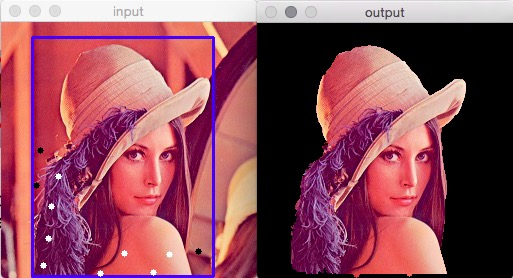
\includegraphics[width=\textwidth]{lena.jpg}
    \caption{Result}
\end{figure}

\section{Conclusion}
In state-of-the-art digital image processing research (reference: http://ipol.im), there are many algorithms based on statistical learning models. Later we should try some signal processing methods in digital image processing.

% \bibliographystyle{plain}
% \bibliography{mybib}


\end{document}
